\documentclass[UTF8]{ctexbeamer}	% Compile at least twice!
%\setbeamertemplate{navigation symbols}{}
\usetheme{Madrid}
% \setbeamertemplate{navigation symbols}{}
% \useinnertheme{rectangles}
% \useoutertheme{infolines}
% \useoutertheme[title,section,subsection=true]{smoothbars}
\useoutertheme{split}
\useinnertheme{rounded}
\setbeamertemplate{headline}{}
\usecolortheme{beaver}


% \usecolortheme{default}
% \usecolortheme{whale}
 
% -------------------
% Packages
% -------------------
\usepackage{
    amsmath,			% Math Environments
    amssymb,			% Extended Symbols
    enumerate,		    % Enumerate Environments
    graphicx,			% Include Images
    lastpage,			% Reference Lastpage
    multicol,			% Use Multi-columns
    multirow,			% Use Multi-rows
    pifont,			    % For Checkmarks
    stmaryrd,            % For brackets
    listings,
    subfigure,
}
\usepackage[english]{babel}
\usepackage{graphicx}
\usepackage{animate}
\usepackage{xeCJK}
\usepackage{fontspec} 
% \setmainfont{KaiTi_GB2312}
% \setCJKmainfont{KaiTi_GB2312}
% \setmainfont{Microsoft YaHei}
% \setCJKmainfont{Microsoft YaHei}
\setmainfont{Source Han Sans SC}
\setCJKmainfont{Source Han Sans SC}

% \newfontfamily\os{Open Sans}
% \newfontfamily\oscl{Open Sans Condensed}
% \newfontfamily\tnr{Times New Roman}
% \newfontfamily\tnrc{Times New Roman Cyr}
% \newfontfamily\tim{Times}
% \newfontfamily\roc{Rockwell}
% \usepackage{CJK}
% \lstset{language=C++}
% \lstset{extendedchars=false}
% \lstset{breaklines}


% -------------------
% Colors
% -------------------
% \definecolor{UniOrange}{RGB}{212,69,0}
% \definecolor{UniGray}{RGB}{62,61,60}
% \definecolor{UniRed}{HTML}{B31B1B}
% \definecolor{UniGray}{HTML}{222222}
% \setbeamercolor{title}{fg=UniGray}
% \setbeamercolor{frametitle}{fg=UniOrange}
% \setbeamercolor{structure}{fg=UniOrange}
% \setbeamercolor{section in head/foot}{bg=UniGray}
% \setbeamercolor{author in head/foot}{bg=UniGray}
% \setbeamercolor{date in head/foot}{fg=UniGray}
% \setbeamercolor{structure}{fg=UniOrange}
% \setbeamercolor{local structure}{fg=black}
% \beamersetuncovermixins{\opaqueness<1>{0}}{\opaqueness<2->{15}}


% -------------------
% Fonts & Layout
% -------------------
% \usepackage{palatino}
\usefonttheme{serif}
% \setbeamerfont{title like}{shape=\scshape}
% \setbeamerfont{frametitle}{shape=\scshape}
% \setbeamertemplate{itemize items}[circle]
% \setbeamertemplate{enumerate items}[default]


% -------------------
% Commands
% -------------------

% Special Characters
% \newcommand{\N}{\mathbb{N}}
% \newcommand{\Z}{\mathbb{Z}}
% \newcommand{\Q}{\mathbb{Q}}
% \newcommand{\R}{\mathbb{R}}
%\newcommand{\C}{\mathbb{C}}

% Math Operators
% \DeclareMathOperator{\im}{im}
% \DeclareMathOperator{\Span}{span}

% Special Commands
% \newcommand{\pf}{\noindent\emph{Proof. }}
% \newcommand{\ds}{\displaystyle}
% \newcommand{\defeq}{\stackrel{\text{def}}{=}}
% \newcommand{\ov}[1]{\overline{#1}}
% \newcommand{\ma}[1]{\stackrel{#1}{\longrightarrow}}
% \newcommand{\twomatrix}[4]{\begin{pmatrix} #1 & #2 \ #3 & #4 \end{pmatrix}}


% -------------------
% Tikz & PGF
% -------------------
\usepackage{tikz}
\usepackage{tikz-cd}
\usetikzlibrary{
    calc,
    decorations.pathmorphing,
    matrix,arrows,
    positioning,
    shapes.geometric
}
\usepackage{pgfplots}
\pgfplotsset{compat=newest}
\usepackage{wrapfig}
\usepackage{cite}


% -------------------
% Theorem Environments
% -------------------
\usepackage{amsthm}
\theoremstyle{plain}
\newtheorem{sit}{Situation}[section]
\newtheorem{prop}{Proposition}[section]
\newtheorem{rtm}{Theorem}[section]
\newtheorem{cor}{Corollary}[section]
\theoremstyle{definition}
\newtheorem{das}{Data structure}[section]
\newtheorem{nex}{Non-Example}[section]
\newtheorem{cla}{class}[section]
\newtheorem{emt}{}[section]
\newtheorem{defn}{Definition}[section]
\theoremstyle{remark}
\newtheorem{rem}{Remark}[section] 
\numberwithin{equation}{section}

\newcommand\caesura{$\mkern -8.5mu\raise -.2ex\hbox{\rotatebox[]{180}{\`}}\ $}
\setbeamertemplate{caption}[numbered]
% -------------------
% Title Page
% -------------------
\title{\textcolor{red}{三维殷集程序进展}}
%\subtitle{\textcolor{white}{Mathematics Conference for the Mysterious and dMagical}}  
\author{谭焱, 邱云昊 
% \newline \newline
%  \small{硕士导师: 王何宇\, \\
%  申请博士导师: 张庆海}
 }

% \institute{\small{现硕士导师: 王何宇 、张庆海 \newline 拟转博士指导教师: 张庆海} \newline   \newline 浙江大学数学科学学院}
\date{\today} 


% -------------------
% Content
% -------------------
\begin{document}
% \begin{CJK}{GBK}{kai}

% Title Page
\begin{frame}
    \titlepage
\end{frame}


\begin{frame}
    \frametitle{提纲}
    \tableofcontents
\end{frame}

\section{程序背景}

% \subsection{\textcolor{red}{}}
\begin{frame}
    \frametitle{殷集研究背景}
    \begin{itemize}
        \item 多相流中的几何和拓扑问题是求解动边界偏微分方程的核心问题.
        \item 现有方法对界面的几何和拓扑问题进行回避,导致了:
              \begin{enumerate}
                  \item 对等距变换的流场不能保证几何性质.
                  \item 对同胚映射的流场不能保证拓扑性质.
                  \item 精度最高为二阶精度.
                  \item 很难对拓扑变化进行严格的处理.
              \end{enumerate}
        \item 我们的核心思想是用\textcolor{red}{几何和拓扑的手段
                  研究几何和拓扑的问题},其中首要工作在于殷集对流相建模.
    \end{itemize}
    \begin{columns}
        \column{0.4\linewidth}<1->
        \centering
        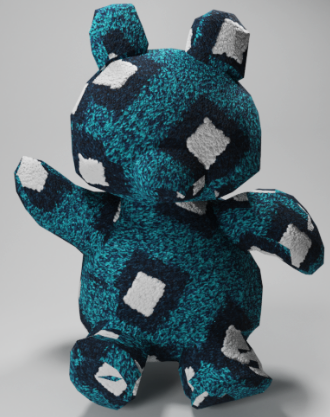
\includegraphics[width = .6\textwidth]{fig/s18.png}
        \column{0.6\linewidth}<1->
        \centering
        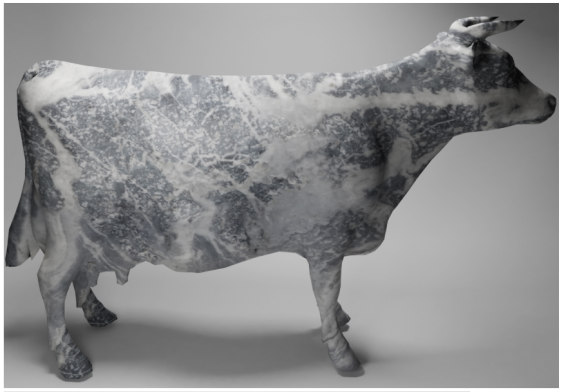
\includegraphics[width = .7\textwidth]{fig/s19.png}
    \end{columns}
\end{frame}


\begin{frame}
    \frametitle{二维殷集}
    \begin{itemize}
        \item \textcolor{red}{殷集}:空间中边界有界的正则半解析开集.所有殷集构
              成的集合被称为殷空间,记为 $\mathbb{Y}$.
        \item 二维空间中,任一个殷集可以唯一表示为
              \[\mathcal{Y} = \cup_j^{\bot \bot}\cap_i \text{int}(\gamma_{j, i} ),\]
              约当曲线 $\gamma_{j, i}$是$\mathcal{Y}$内第$j$个连通分量
              的第$i$条边界.
        \item 实现了殷集上的布尔代数.
    \end{itemize}
    \begin{figure}[!htb]
        \centering
        \subfigure{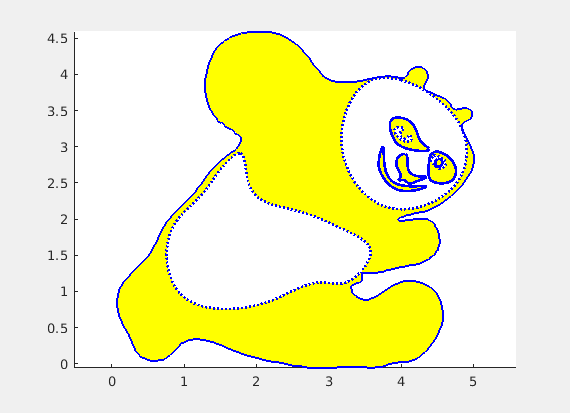
\includegraphics[width=0.3\textwidth]{fig/p.png}}
        \subfigure{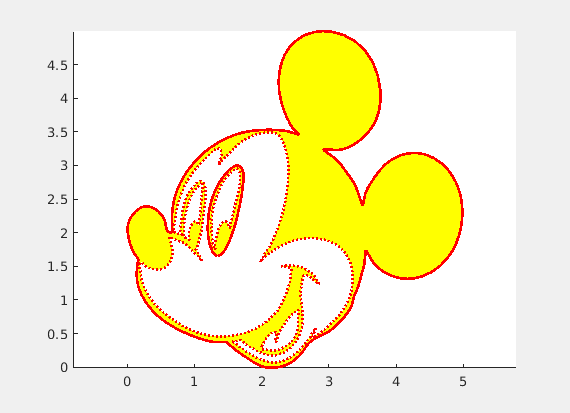
\includegraphics[width=0.3\textwidth]{fig/m.png}}
        \subfigure{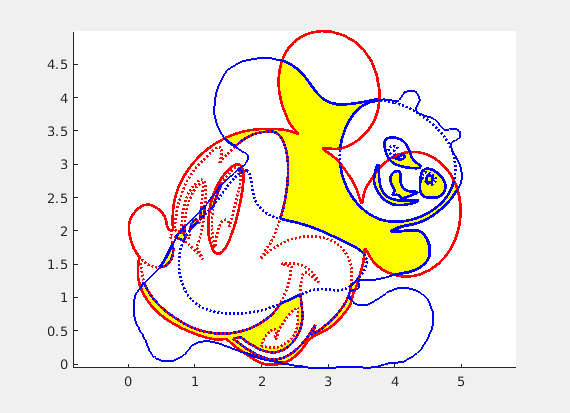
\includegraphics[width=0.3\textwidth]{fig/pm.png}}
        \caption{二维殷集的交}
        %   \vspace{0.2in}
    \end{figure}
\end{frame}

\begin{frame}
    \frametitle{三维殷集}
    \begin{itemize}
        \item
              \textcolor{red}{二流形的分类定理} \newline
              有向的紧二流形是同胚于球或者圆环或它们的有限个连通和.
              \begin{figure}[!htb]
                \centering
                \subfigure{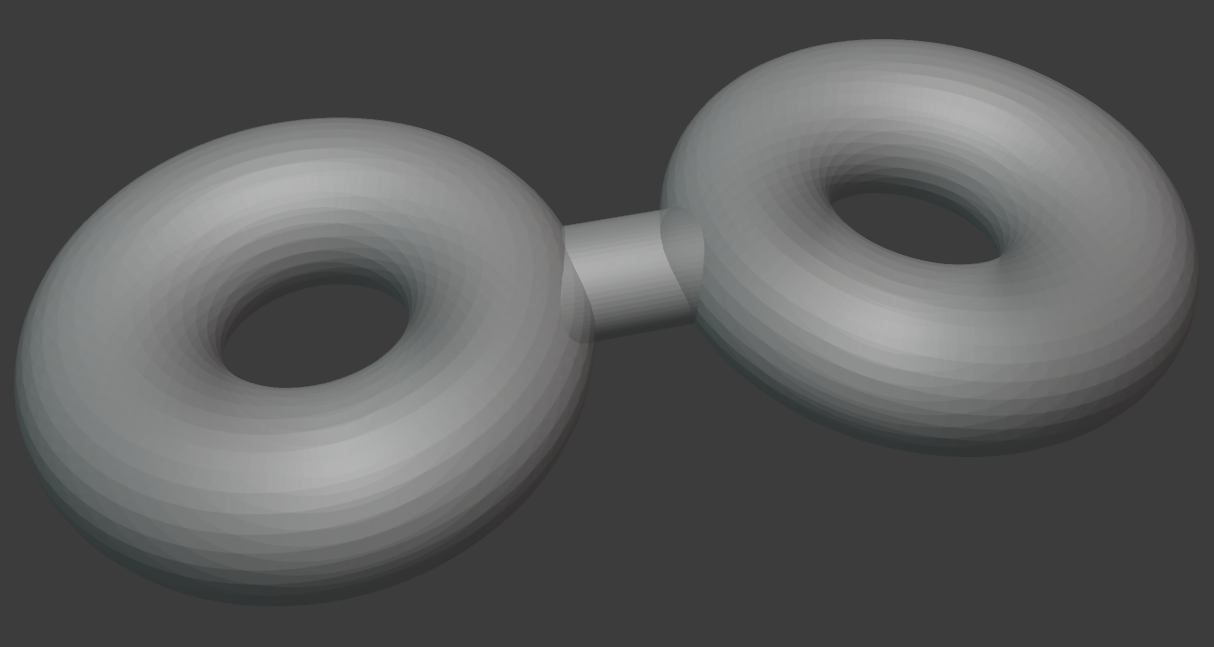
\includegraphics[width=0.4\textwidth]{fig/connectsum.png}} \qquad
                \subfigure{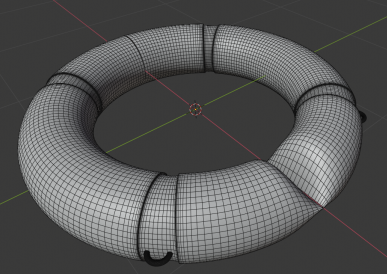
\includegraphics[width=0.3\textwidth]{fig/past.png}}
            \end{figure}


        \item 黏合紧曲面是一个二维连通紧流形或这种流形的商空间, 其商映射
              将多个与一维 CW 复形同胚的子集粘在一起; 将这个一维子集删除后
              该黏合紧曲面仍然是连通的.
    \end{itemize}
\end{frame}

\begin{frame}
    \frametitle{三维殷集的唯一表示}
    \begin{itemize}
        \item 任一个殷集$\mathcal{Y} \in \mathbb{Y}$可以唯一表示为
              \[\mathcal{Y} = \cup_j^{\bot \bot} \cap_i \text{int}(\Gamma_{j, i}),\]
              黏合紧曲面$\Gamma_{j, i}$是$\mathcal{Y}$的第$j$个连通分量的第$i$个边界.
        \item 唯一表示中每个内部是有界区域的黏合紧曲面对应一个连通分量.

        \item 连通分量的边界中每个内部无界的曲面对应连通分量闭包的洞.
    \end{itemize}
    \begin{columns}
        \column{0.4\linewidth}<1->
        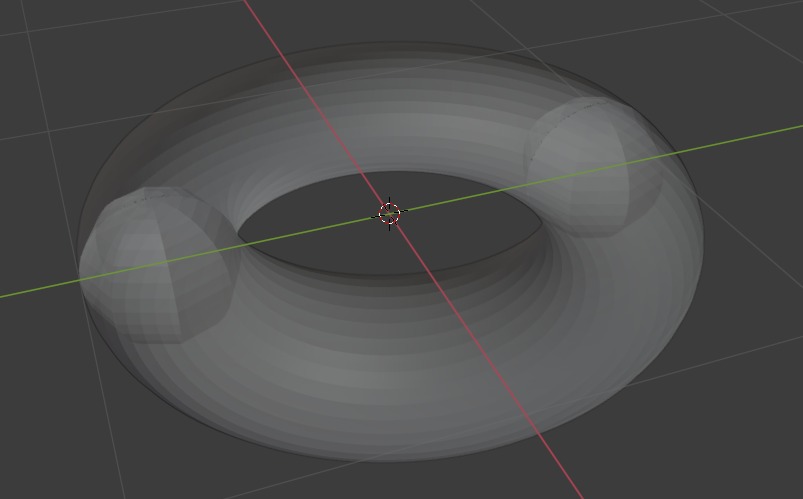
\includegraphics[width = \textwidth]{fig/s1.png}
        \column{0.4\linewidth}<1->
        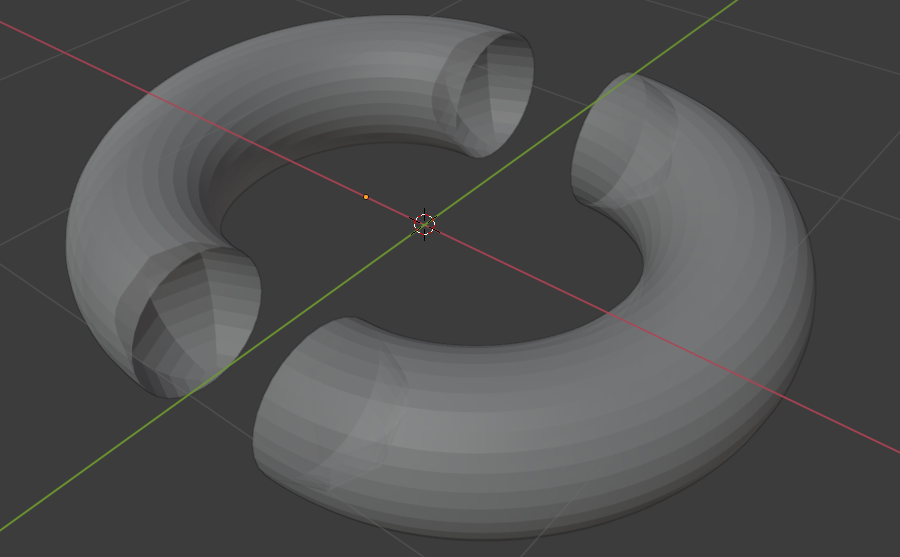
\includegraphics[width = \textwidth]{fig/s2.png}
    \end{columns}
\end{frame}

\section{程序进展}
\subsection{程序架构}
\begin{frame}
    \frametitle{程序的实现方式}
    \begin{itemize}
        \item 实现步骤
    \begin{enumerate}
        \item 计算殷集边界上的所有非流形点.
        \item 沿非流形点剪开黏合紧曲面得到若干曲面片.
        \item 根据交并补的需要删除曲面片或改变曲面片方向.
        \item 将曲面片重新粘合成黏合紧曲面集合.
        \item 黏合紧曲面集合唯一表示一个三维殷集作为布尔运算结果.
    \end{enumerate}

        \item 代码模块
        \begin{enumerate}
            \item class TriangleIntersection.
            \item class Triangulation. 找到非流形点.
            \item class Prepast. 生成曲面片.
            \item class RemoveOverlap.
            \item class Locate. 恰当的保留曲面片.
            \item class Past. 生成黏合紧曲面.
            \item YinSet(). 构造殷集.
        \end{enumerate}
    \end{itemize}
\end{frame}

\begin{frame}
    \frametitle{时间瓶颈分析}
    \begin{itemize}
        \item 求交运算在同一图形的不同加密次数的模型上计算时间.
        \begin{table}[]
            \resizebox{0.9\textwidth}{!}{%
            \begin{tabular}{|l|l|l|l|l|l|l|}
            \hline
            三角形/个 & 三角形求交/秒 & Ratio & 三角化/秒 & Ratio & 总时间 & Ratio \\ \hline
$2.11 \times 10^3$ & $5.52 \times 10^{-1}$ &      & $1.63 \times 10^{-1}$ &  & $7.63 \times 10^{-1}$ &
\\ \hline
$3.46 \times 10^4$ & $1.04 \times 10^{2}$  & 1.87 & $2.33 \times 10^{0}$  & 0.95 & $1.07 \times 10^{2}$  & 1.76
\\ \hline
$1.14 \times 10^5$ & $1.26 \times 10^{3}$  & 2.09 & $7.66 \times 10^{0}$  & 0.99 & $1.27 \times 10^{3}$  & 2.07
\\ \hline
$3.59 \times 10^5$ & $1.28 \times 10^{4}$  & 2.02 & $2.42 \times 10^{1}$  & 1.00 & $1.29 \times 10^{4}$  & 2.02
\\ \hline
$5.39 \times 10^5$ & $2.89 \times 10^{4}$  & 2.00 & $3.59 \times 10^{1}$  & 0.97 & $2.90 \times 10^{4}$  & 1.99
\\ \hline
            \end{tabular}
            }
            \end{table}

            \item 计算时间过长,瓶颈在三角形求交,需求
            时间复杂度更低的求交算法.
            
            \item 三角化的时间复杂度达到理论最优的$O(1)$,.
    \end{itemize}
\end{frame}

\subsection{计算非流形点的优化}
\begin{frame}
    \frametitle{使用空间划分降低求交计算时间度}
    \begin{itemize}
        \item 三角形相交局部发生, 将三角形划分到不同的局部降低计算量.
        \begin{center}
            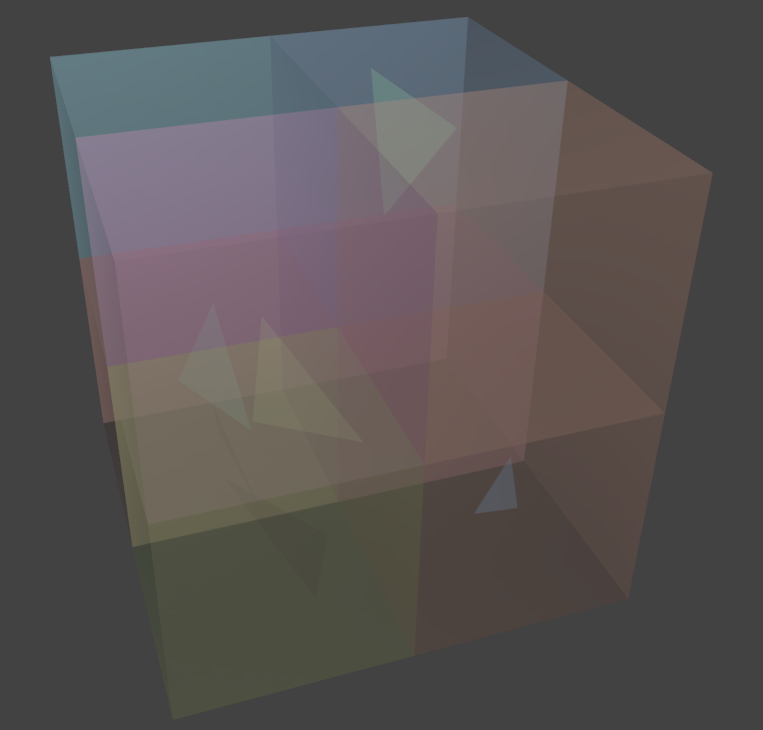
\includegraphics[width = 0.3\textwidth]{fig/tree.png}
        \end{center} 
        \begin{table}[]
            \resizebox{0.7\textwidth}{!}{%
            \begin{tabular}{|l|l|l|l|l|}
            \hline
            三角形/个 & 俩俩求交/秒 & Ratio & 空间划分/秒 & Ratio \\ \hline
$2.11 \times 10^3$ & $5.52 \times 10^{-1}$ &      & $4.26 \times 10^{-1}$ & 
\\ \hline
$3.46 \times 10^4$ & $1.04 \times 10^{2}$  & 1.87 & $5.14 \times 10^{0}$  & 0.89 
\\ \hline
$1.14 \times 10^5$ & $1.26 \times 10^{3}$  & 2.09 & $1.36 \times 10^{1}$  & 0.82 
\\ \hline
$3.59 \times 10^5$ & $1.28 \times 10^{4}$  & 2.02 & $3.44 \times 10^{1}$  & 0.80 
\\ \hline
$5.39 \times 10^5$ & $2.89 \times 10^{4}$  & 2.00 & $4.85 \times 10^{1}$  & 0.84 
\\ \hline
            \end{tabular}
            }
            \end{table}
    \end{itemize}
\end{frame}

\begin{frame}
    \frametitle{针对殷集与网格求交优化}
    \begin{itemize}
        \item 有限体积法基于网格的控制体,求解需大量控制体和计算域求交.
        \item 不妨假设三角形与至多常数$N$个网格面相交.
        \item 计算复杂度从$O(n_1 * n_2)$降为$O(n_2)$.
        \item 只需替换TriangleIntersection模块.
        \vspace{0.2in}
         \begin{columns}
        \column{0.4\linewidth}<1->
        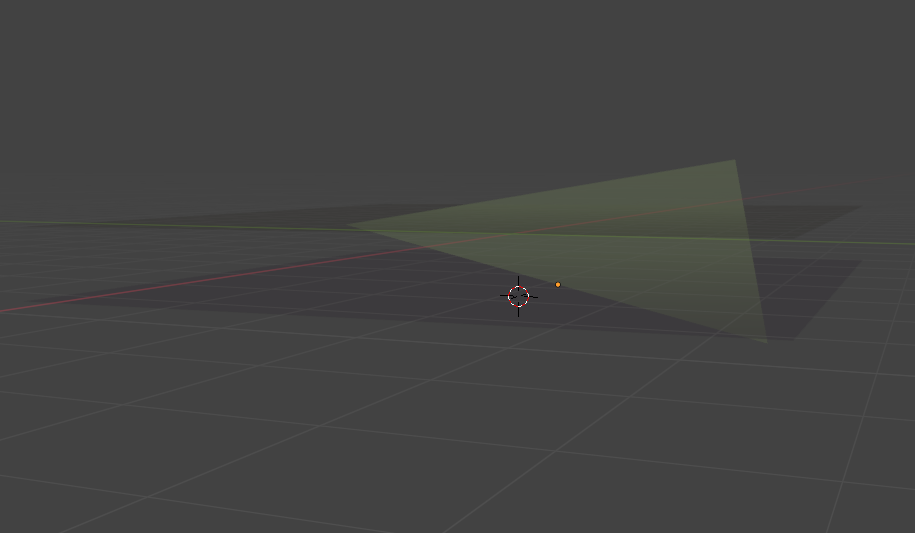
\includegraphics[width = \textwidth]{fig/sw.png}
        \column{0.4\linewidth}<1->
        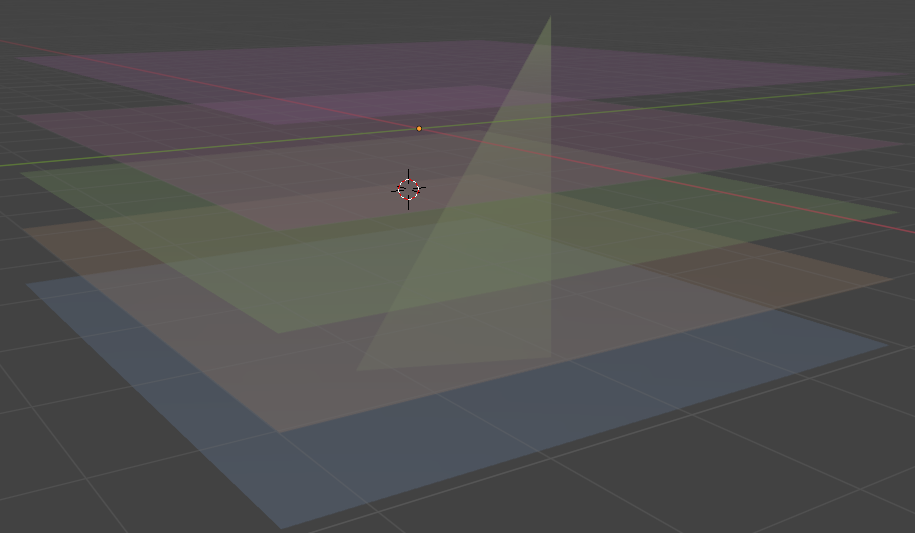
\includegraphics[width = \textwidth]{fig/sw2.png}
    \end{columns}
    \end{itemize}
\end{frame}

\subsection{粘合模块的修改}
\begin{frame}
    \frametitle{原Past方法的问题}
    \begin{itemize}
        \item 原Past方法只证明了能将殷集正确黏合.
        \item 无法检测到一些疑似殷集的非殷集输入.
        \vspace{0.2in}
        \begin{columns}
       \column{0.5\linewidth}<1->
       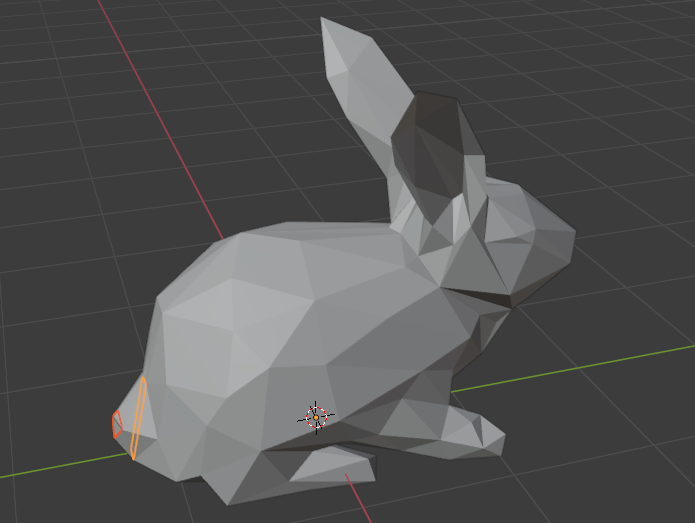
\includegraphics[width = \textwidth]{fig/rabbit1.png}
       \column{0.5\linewidth}<1->
       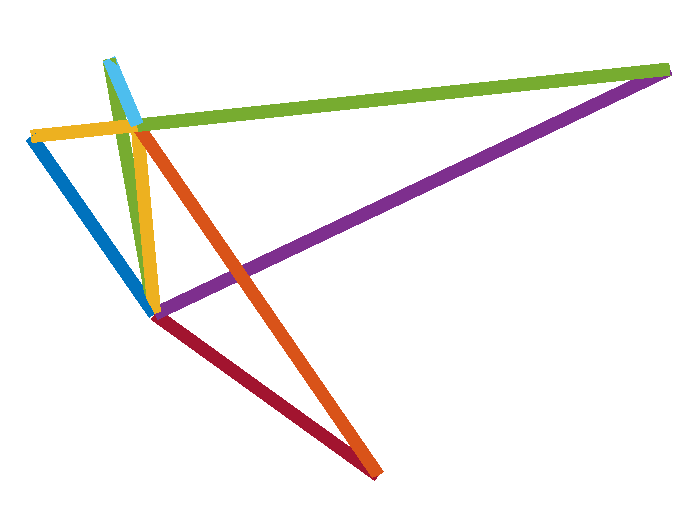
\includegraphics[width = \textwidth]{fig/rabbit2.png}
   \end{columns}
    \end{itemize}
\end{frame}

\begin{frame}
    \frametitle{黏合紧曲面的性质}
    \begin{center}
        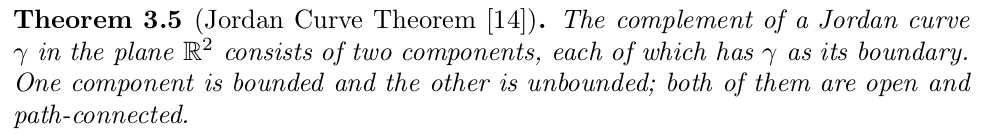
\includegraphics[width = 0.9\textwidth]{fig/jordancurve.png}
    \end{center}
        \begin{itemize}
            \item 黏合紧曲面同样拥有类似性质.
            \vspace{0.2in}
            \begin{center}
                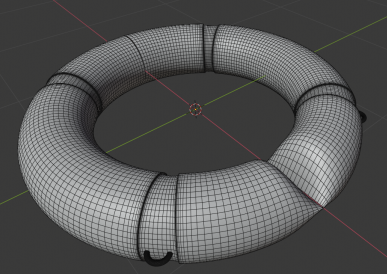
\includegraphics[width = 0.5\textwidth]{fig/past.png}
            \end{center}
        \end{itemize}
\end{frame}

\begin{frame}
    \frametitle{生成黏合紧曲面的方法}
    \begin{center}
        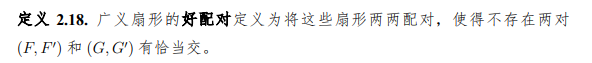
\includegraphics[width = 0.9\textwidth]{fig/goodpair.png}
    \end{center}
    \vspace{-0.1in}
    \begin{itemize}
        \item 好配对粘合可以得到一个连通分量的边界.
        \item 正向好配对粘合再反向好配对粘合得到黏合紧曲面.
        \item 该方法检测到Rabbit不为殷集.
    \end{itemize}
     \begin{columns}
        \column{0.39\linewidth}<1->
        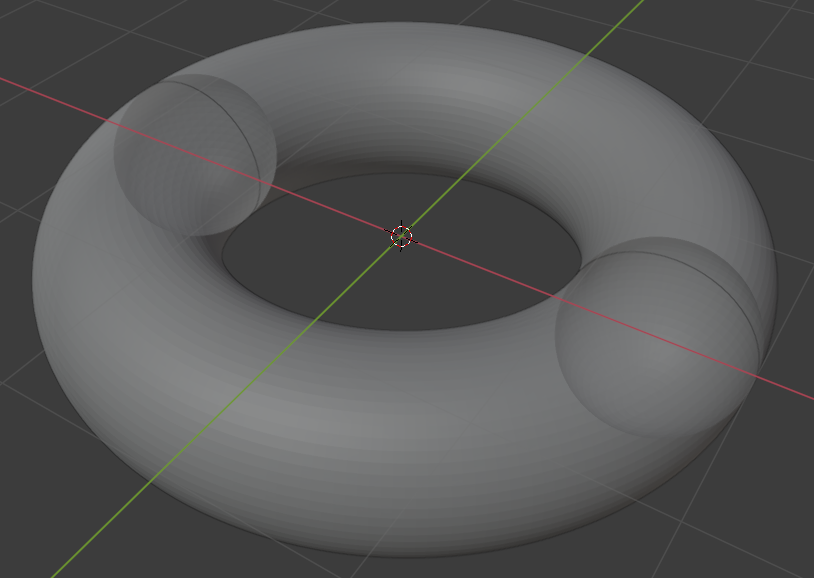
\includegraphics[width = \textwidth]{fig/s3.png}
        \column{0.4\linewidth}<1->
        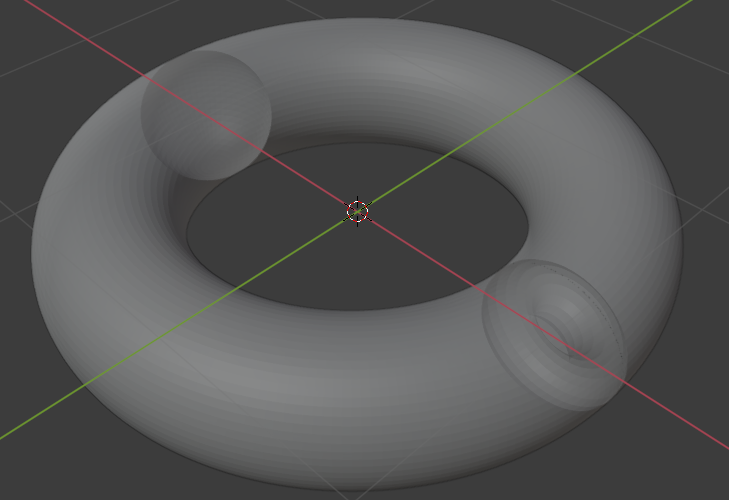
\includegraphics[width = \textwidth]{fig/s31.png}
    \end{columns}
\end{frame}

\section{后续工作}
\begin{frame}
    \frametitle{现有测试模型的问题}
    \begin{columns}
        \column{0.3\linewidth}<1->
        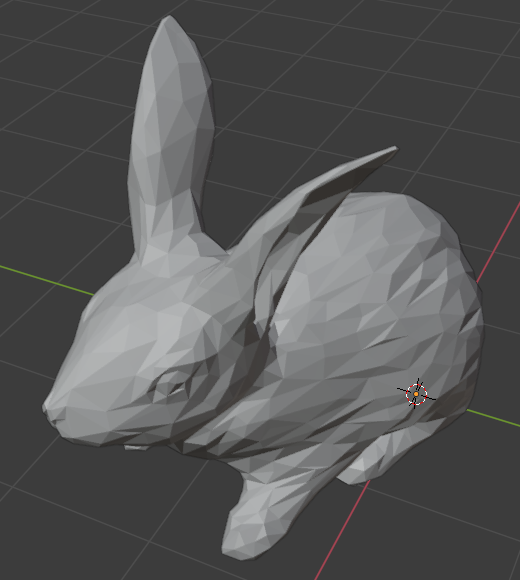
\includegraphics[width = \textwidth]{fig/wrong1.png}
        \column{0.3\linewidth}<1->
        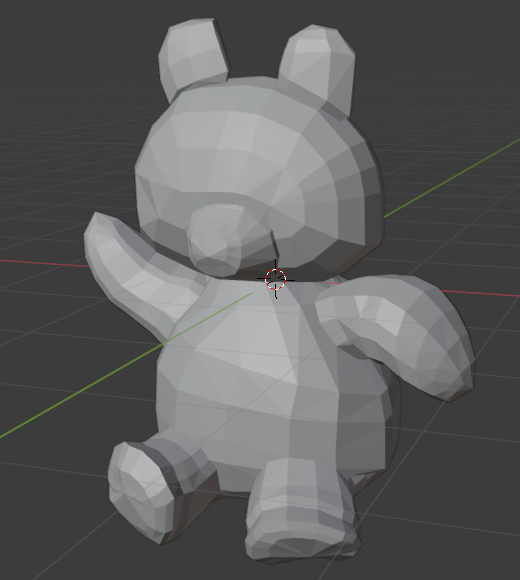
\includegraphics[width = \textwidth]{fig/wrong2.png}
        \column{0.32\linewidth}<1->
        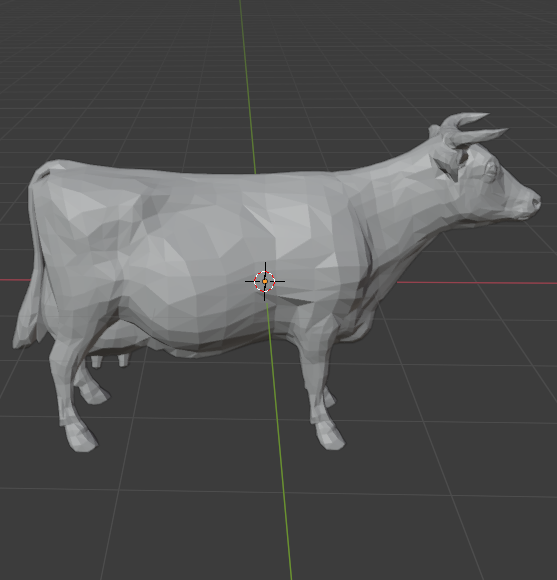
\includegraphics[width = \textwidth]{fig/wrong3.png}
    \end{columns}
    \begin{columns}
        \column{0.65\linewidth}<1->
    \begin{enumerate}
        \item Rabbit与Teddy内部洞边界的方向朝外.
        \item cow尾部有不可定向的曲面片.
        \item 缺乏几何结构复杂的殷集测试模型.
    \end{enumerate}
    \column{0.3\linewidth}<1->
        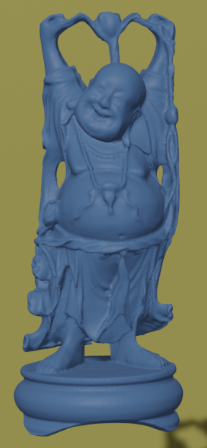
\includegraphics[width = 0.4
        \textwidth]{fig/wrong4.png}
    \end{columns}

\end{frame}

\begin{frame}
    \frametitle{后续工作方向}
    \begin{itemize}
        \item 增加测试样例.
        \begin{enumerate}
        \item 熟悉已完成的三维殷集表面建模程序.
        \item 截取简单殷集模型在复杂流场运行一段时间后的殷集.
        \item 使用blender构建拓扑结构复杂的模型.
        \item 验证程序的正确性.
    \end{enumerate}
    
    \item 分析优化计算非流形点.
    \begin{enumerate}
        \item 分析布尔运算程序速度是否为瓶颈.
        \item 检索更优的三角形求交和三角化算法.
    \end{enumerate}

    \item 重构现有程序.
    \end{itemize}
\end{frame}


\section*{}
\begin{frame}
    \centering\huge
    \textcolor{red}{请老师同学批评指正!}
\end{frame}
\end{document}